\chapter{Top-2$m$ XOR Thompson Sampling}

In this chapter we will both present and analyze our suggested generalization of Russo's Top-Two Thompson sampling: Top-2$m$ XOR Thompson sampling. The underlying idea still revolves around repeatedly apllying Thompson sampling until two different candidates are at hand.

\Cref{section:algorithm} introduces the algorithm and provides some explanations with regards to generalization decisions. It also introduces the constraint $\psi_{S^*} = \frac{1}{2}$. Subsequently, \Cref{section:analysis} analyzes properties of the algorithm. In particular it presents bounds on the measurement plan, states general consequences of finite measurement and discusses implications of underallocation and overallocation. We firmly believe that all of those are very useful to show that this algorithm's measurement plan converges to the optimal constrained measurement plan $\psi^{\frac{1}{2}*}$. Proofs for those statements are provided in \Cref{section:txts_proofs}. Additionally, we provide some empirical results in \Cref{section:empirical_behavior}.

\section{Algorithm}\label{section:algorithm}
As a generalization of Russo's TTTS, the main difference lies in the fact that candidates are sets. Hence Thompson sampling is repeated until set inequality is reached. However, we can only ever sample individual arms, i.e. not sets. Hence in this set scenario, we still need a mechanism to select a single arm from a set. Therefore, when generalizing Russo's approach, the central and unavoidable question arises: 'How to select a single arm from two unequal set candidates?'

According to a suggestion Russo gives in his outlook, we decided to tackle this question by splitting it up into two steps.

First, given candidates $S_1$ and $S_2$ with $S_1 \neq S_2$, we compute the set of elements which are contained in exactly one of both sets, i.e. the XOR of both sets. Naturally, this restricted set is of cardinality at least 2. Intuitively it points us towards arms which are 'uncertain'. Observe that arms which are clearly suboptimal are very unlikely to appear in either $S_1$ or $S_2$ through Thompson sampling. At the same time, arms that are clearly optimal are very likely to appear in both $S_1$ and $S_2$ through Thompson sampling. Hence arms that appear in only either of them are neither clearly optimal nor clearly suboptimal.

As mentioned before, the XOR of $S_1$ and $S_2$ will always contain at least two elements. Hence we need to define an approach on how to select from the XOR. According to both Russo's suggestion as well as Occam's razor, we opted for uniform selection.

We believe that the applying a XOR to both candidates is essential for the correctness of the algorithm, whereas the uniform sampling from the XOR of both candidates could easily be substituted by other distributions. We would expect such a change to preserve correctness, as long as every arm of the XOR is sampled with strictly positive probability. Yet, it would likely alter the hyperparamter $\beta = \psi_{S^*}$.

We present the approach to sample an arm in step $n + 1$ in \Cref{alg:TXTS}. This approach can be repeated either for a fixed amount of samples or until a specific confidence level is reached. Note that the confidence level can be approximated in every step. The confidence level is equal to $\Pi_n(\Theta_S)$ where $S = \argmax_{S'} \Pi_n(\Theta_{S'})$. Concretely, this quantity can be estimated by drawing samples from $\Pi_n$ and identifying for which set $S$ the fraction $\frac{\text{\# samples in which $S$ is optimal}}{\#samples}$ is largest. The fraction of this $S$ approximates the confidence level.
\begin{algorithm}[H]
  \caption{Given a posterior $\Pi_n$ in step $n+1$}
  \label{alg:TXTS}
  \begin{algorithmic}
    \State $\hat{\theta} \sim \Pi_n$
    \State $S_1 =$ top-$m(\hat{\theta})$
    \Repeat
      \State $\hat{\theta} \sim \Pi_n$
      \State $S_2 = $ top-$m(\hat{\theta})$
    \Until{$S_1 \neq S_2$}
    \State $I_{n+1} \sim \mathcal{U}(S_1 \oplus S_2)$
    \State Play $I_{n+1}$, observe reward and update posterior
  \end{algorithmic}
\end{algorithm}
We expect this algorithm to induce a measurement plan $\psi$ such that $\psi_{S^*} = \frac{1}{2}$. This expectation gives rise to the constrained optimization from the previous chapter. Note that this constraint is a consequence of the design decision of which operation to apply to candidates $S_1$ and $S_2$.

\section{Analysis}\label{section:analysis}
Starting off by a statement about the implications of finite measurement, we later establish bounds and equalities on the measurement plan $\psi$ of the algorithm.

The following lemma formalizes two three seemingly intuitive statements. First, it shows that for each arm that is sampled infinitely many times, the estimated mean will converge to its true mean. Second, it demonstrates that if every arm is sampled infinitely often, the posterior will put all of its mass on parameters with $S^*$ as top-$m$ arms. Third, it argues that as long as some arms have only been granted finite measurement, they can't be ruled out from being optimal.
\begin{lemma}\label{lemma:finite_measurement}
  $\mathcal{I} = \{l: \sum_{n=1}^\infty \psi_{n, l} < \infty\}$
  \begin{itemize}
    \item $\forall l \notin \mathcal{I}, \forall \epsilon: \Pi_n(\{\theta: \theta_l \in (\theta^*_l - \epsilon, \theta^*_l + \epsilon)\}) \rightarrow 1$
    \item $\mathcal{I} = \emptyset \Rightarrow
    \alpha_{n, S} \rightarrow \begin{cases}
      1 & \text{if } S = S^*\\
      0 & \text{if } S \neq S^*
    \end{cases}$
    \item $\forall S \subset \mathcal{I}: \liminf_{n \rightarrow \infty} \alpha_{n, S} > 0$
  \end{itemize}
\end{lemma}
Going on to expressing the measurement plan, we observe that a closed-form equality is not easy to obtain. In comparison to Russo's case, it is much harder to construct a closed-form probability of arm $l$ being sampled in a given step as there are many more different scenarios. Vaguely speaking, the XORs can be of very different kinds.

In this spirit, we offer both lower and upper bounds on the measurement plan of a single arm. The overall idea is to case-distinguish if $l$ lies set $S_1$ or $S_2$. Facing the probability of $l$ being selected given its belonging to the XOR, we leverage the knowledge of the uniform draw. Hence we have $\Pr[I_n = l|l \in S_1 \oplus S_2] = \frac{1}{|S_1 \oplus S_2|}$. The cardinality of the XOR can be trivially bounded from below by 2 or from above by 2$m$. Note that these inequalities are tight with respect to $n$ as $m$ can be seen as a constant.
\begin{proposition}\label{proposition:measurement_plan_arm}
  \begin{align}
    \psi_{n, l} &\leq \frac{1}{2}(\sum_{S: l \in S} \frac{\alpha_{n, S}}{1 - \alpha_{n, S}} (1 - \alpha_{n, l}) +  \sum_{S': l \notin S'} \frac{\alpha_{n, S'}}{1 - \alpha_{n, S'}} \alpha_{n, l}) \\
    \psi_{n, l} &\geq \frac{1}{2m}(\sum_{S: l \in S} \frac{\alpha_{n, S}}{1 - \alpha_{n, S}} (1 - \alpha_{n, l}) +  \sum_{S': l \notin S'} \frac{\alpha_{n, S'}}{1 - \alpha_{n, S'}} \alpha_{n, l})
  \end{align}
\end{proposition}
Having established bounds on the measurement plan for individual arms, we proceed to establish two equalities on the measurement plan for sets. In this case we neither propose a closed-form solution nor a bound. Rather, we veil some of the uncertainty with a probability term, which turns out to be sufficiently expressive for some of the later applications.
\begin{proposition}\label{proposition:measurement_pan_set}
  \begin{align}
    \psi_{n, S} &= \frac{1}{2} \alpha_{n, S} +  \Pr[I_n \in S | S_1 \neq S] (1 - \alpha_{n, S}) \\
    \psi_{n, S} &= \frac{\alpha_{n, S}}{2} +  \frac{\alpha_{n, S}}{2} \sum_{S'\neq S} \frac{\alpha_{n, S'}}{1 - \alpha_{n, S'}} + \Pr[S_1, S_2 \neq S \wedge I_n \in S]
  \end{align}
\end{proposition}
This form of $\psi_{n, S}$ allows us to deduct that the algorithm collects infinite measurement on every arm given infinite samples.
\begin{lemma}\label{lemma:infinite_measurement}
  \begin{align}
    \sum_{n \in \mathbb{N}} \psi_{n, S} \rightarrow \infty
  \end{align}
\end{lemma}
Recalling \Cref{lemma:finite_measurement}, this is particularly interesting as it signals that for $n \rightarrow \infty$ we have that $\mathcal{I} = \emptyset$. Therefore $\alpha_{n, S^*} \rightarrow 1$ holds true, too.
Having established $\psi_{n, S}$ as function of $\alpha_{n, S}$, we continue by analyzing the effect of $\alpha_{n, S} \rightarrow 1$ on $\psi_{n, S}$, for general $S$, followed by the application on $S^*$.
\begin{lemma}\label{lemma:psi_convergence}
  \begin{align}
    \alpha_{n, S} \rightarrow 1 \Rightarrow \psi_{n, S} \rightarrow \frac{1}{2}
  \end{align}
\end{lemma}
This result confirms our hunch about the constraint induced of the algorithm: once it becomes 'sure' of the optimality of a set $S$, it will sample arms from it with probability $\frac{1}{2}$. As we have previously argued, we have that $\alpha_{n, S^*} \rightarrow 1$ and therefore $\psi_{n, S^*} \rightarrow \frac{1}{2}$.

Moreover, once we know that $\alpha_{n, S^*} \rightarrow 1$, we can simplify the bound from \Cref{proposition:measurement_plan_arm}.
\begin{lemma}\label{lemma:measurement_plan_bound_max}
  If $\alpha_{n, S^*} \rightarrow 1$, then for all $i \notin S^*$ and for all $j \in S^*$:
  \begin{align}
    \psi_{n, i} &\leq \frac{\alpha_{n, i}}{\max_{S' \neq S^*} \alpha_{n, S'}} \\
    \psi_{n, j} &\leq \frac{1 - \alpha_{n, j}}{\max_{S' \neq S^*} \alpha_{n, S'}}
  \end{align}
\end{lemma}

\section{Empirical behavior}\label{section:empirical_behavior}
%What true distributions are assumed?
%What prior and posterior distributions are assumed?
%How is C computed?
%How is alpha computed, as it is defined via a huge integral?
%How is psi computed, as there is no closed form?

TODO: Talk about updates of priors.

For the following empirical results we assumed the rewards of arms to follow Bernoulli distributions with means $\theta^* = [.1, .2, .3, .4, .5, .6, .7, .8, .9]$. We defined priors/posteriors to be Beta distributed with initial parameters $\alpha = \beta = 1$, mimicking a uniform prior on the set of arms.

The posterior mass put on certain events, in particular the confidence, were computed as described in \Cref{section:algorithm}. \Cref{fig:confidences} indicates the confidence for a given number of steps of our method compared to the the uniform allocation and Thompson sampling.

\begin{figure}[h]
  \centering
  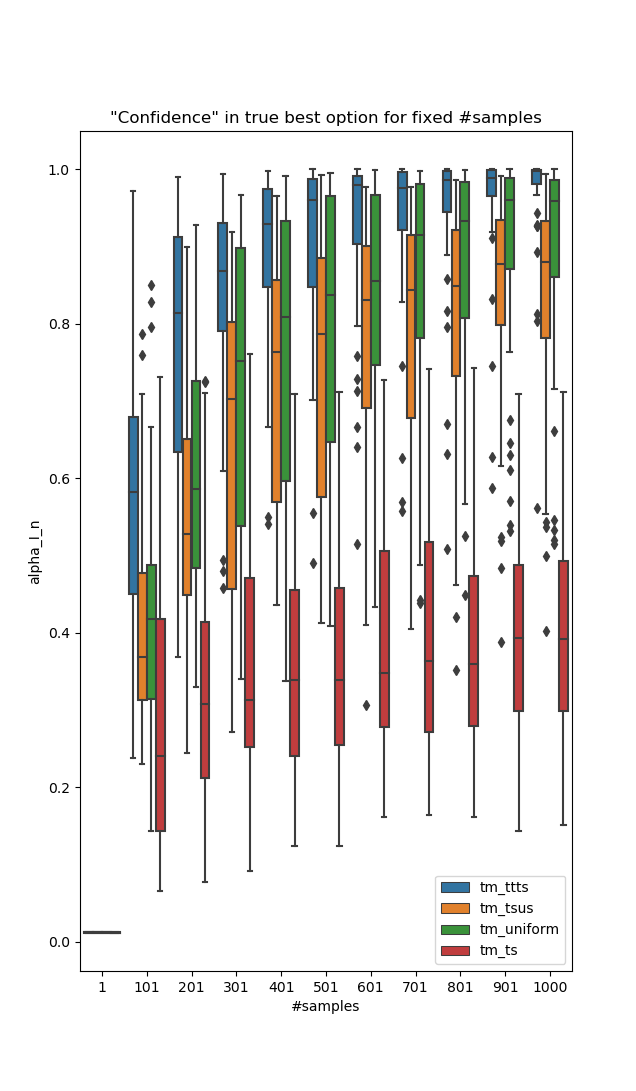
\includegraphics[width=.5\textwidth]{190723-confidences.png}
  \caption{Unconstrained and constrained optimal allocation for $\theta_1$ and $\theta_2$, top-4}
  \label{fig:confidences}
\end{figure}

As we don't have a closed form for the average measurement plan $\bar{psi}_{n,l}$ at our disposal, we approximate it with the empirical sampling frequencies. \Cref{fig:measurement_plan} indicates said empirical sampling frequencies. Note that $\bar{psi}_{S^*}$ can nicely be read to equal $\frac{1}{2}$.

\begin{figure}[h]
  \centering
  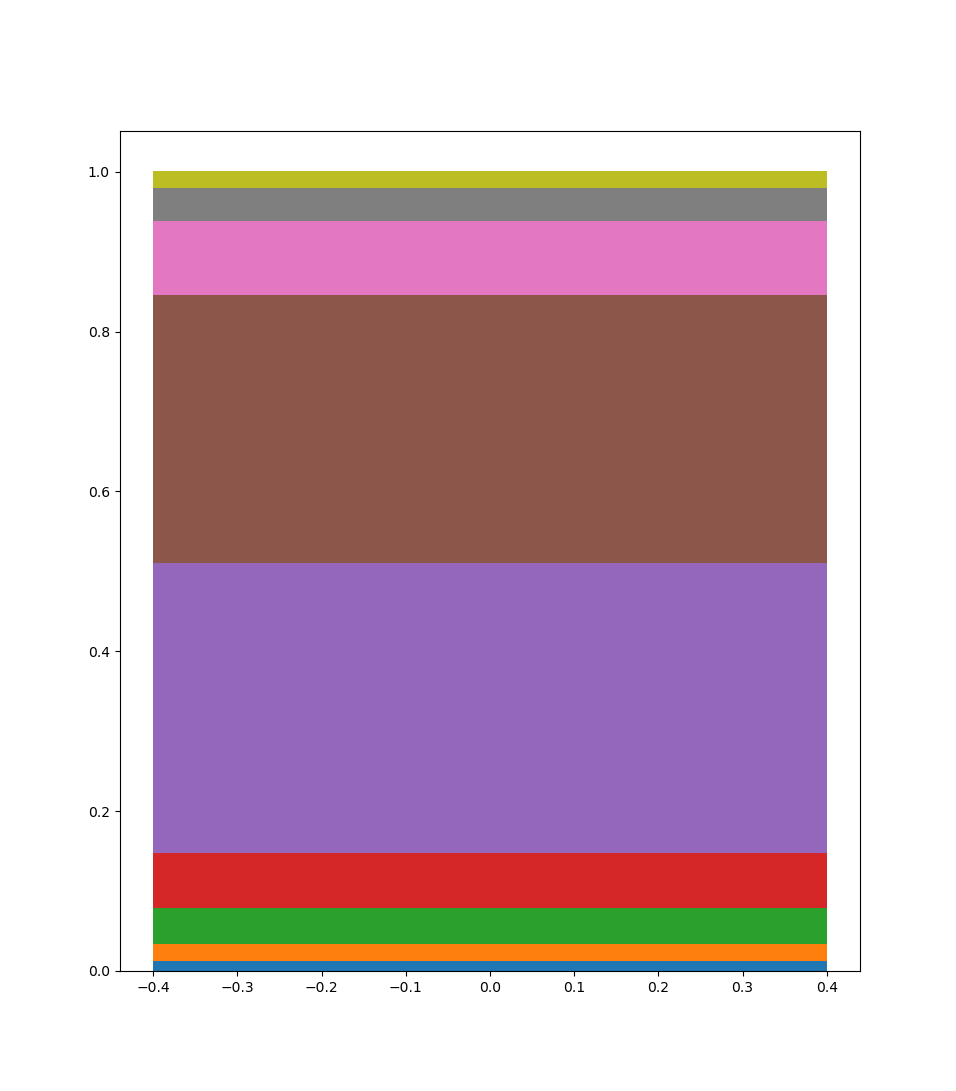
\includegraphics[width=\textwidth]{190723-selections_2.png}
  \caption{Unconstrained and constrained optimal allocation for $\theta_1$ and $\theta_2$, top-4}
  \label{fig:measurement_plan}
\end{figure}

As we know from \Cref{section:optimal_statements}, the optimal allocation gathers equal evidence for all pairs from $S^* \times S^{*c}$. We used the empirical sampling frequencies to approximate those coefficients. A qualitative comparison of the individual coefficients can be found in \Cref{fig:algorithm_coefficients}. The individual $C_{j, i}$ were computed just as described in \Cref{section:concrete_optimal_allocation}.

\begin{figure}[h]
  \centering
  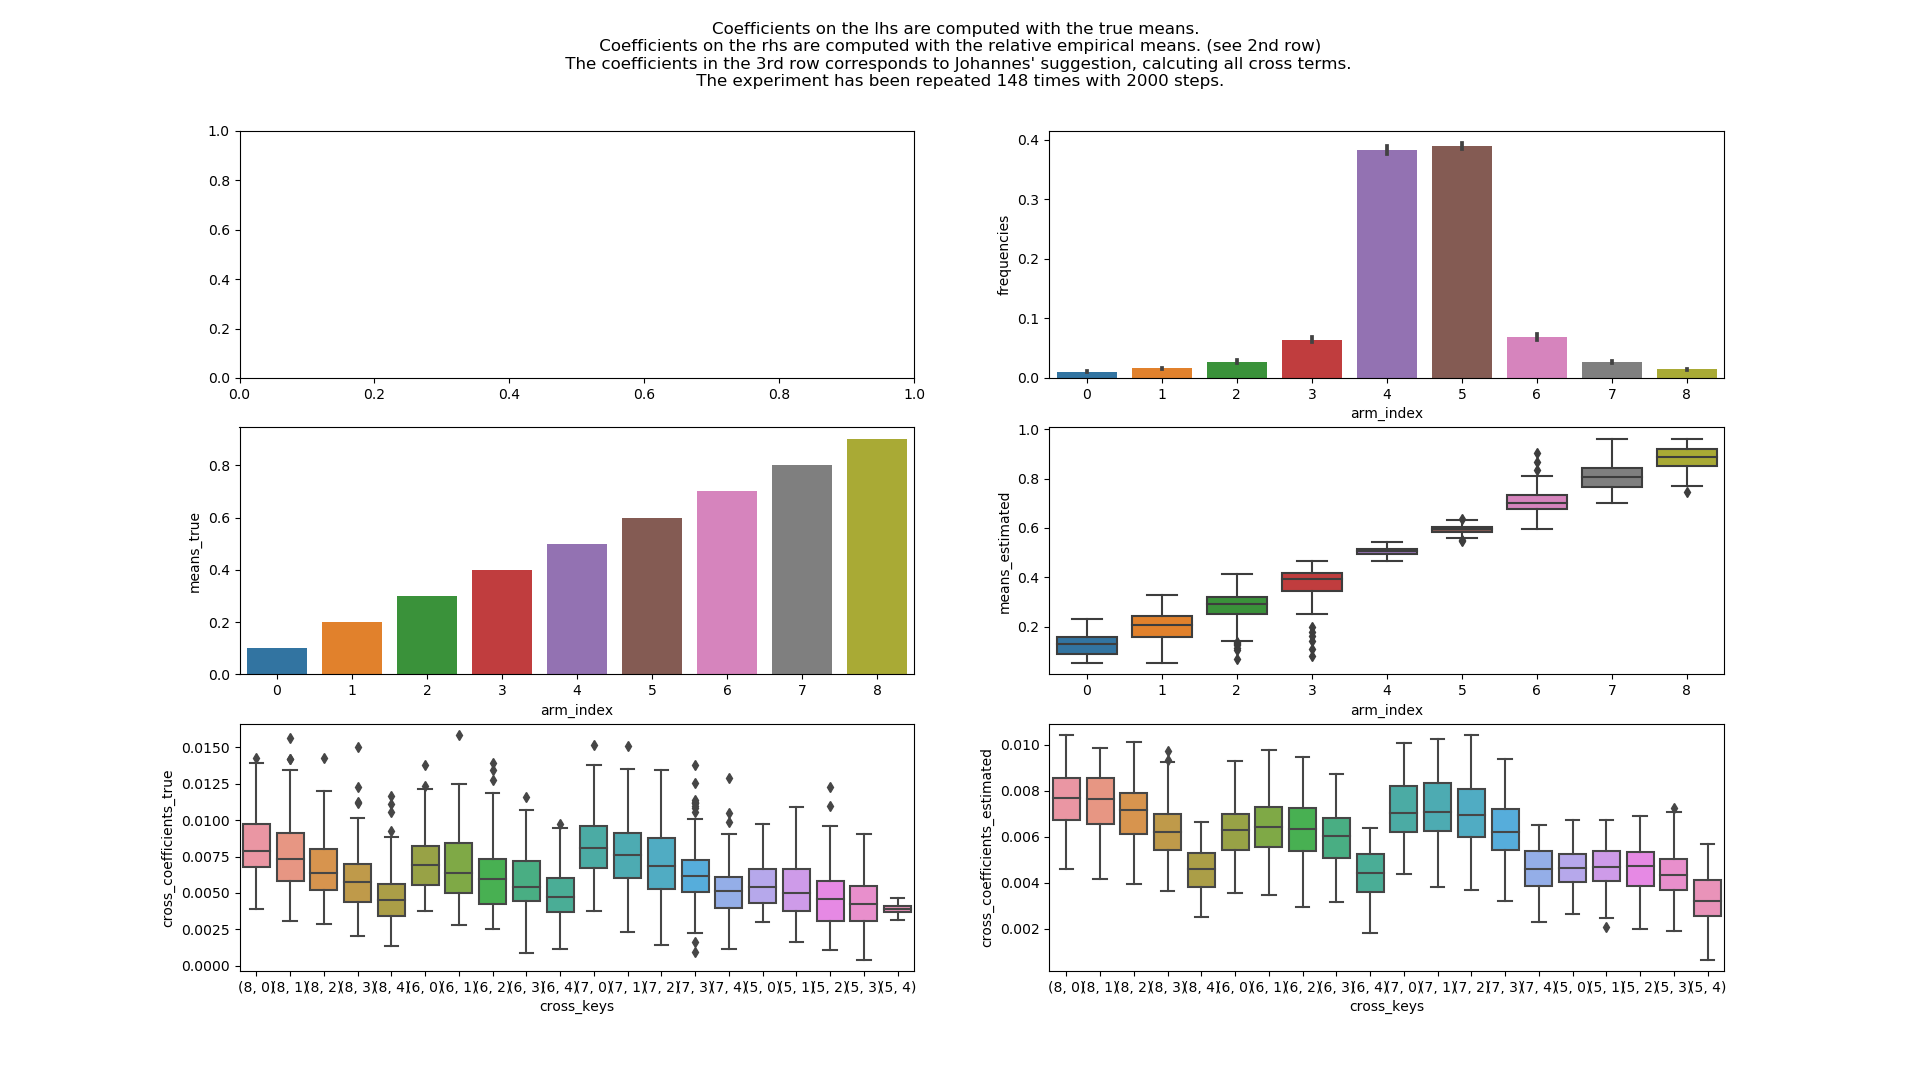
\includegraphics[width=\textwidth]{190909-coefficients_2000.png}
  \caption{Unconstrained and constrained optimal allocation for $\theta_1$ and $\theta_2$, top-4}
  \label{fig:algorithm_coefficients}
\end{figure}

\section{Further results}

\begin{lemma}\label{lemma:limsup_undersampling}
  Given $\sum_n(\frac{1}{2} - \psi_{l, n}) \mathbb{I}[\psi_{l, n} \leq \psi_l^* - \delta] < \infty$ we have that
  \[\limsup \bar{\psi}_{l, n} \geq \psi_j^* \text{ and } \liminf \bar{\psi}_{l, n} \geq \psi_j^*\]
\end{lemma}

\begin{lemma}\label{lemma:psi_undersampled}
  \begin{align}
    \psi_{n, \hat{j}} \geq \frac{1}{2} - m\exp(-n \delta)
  \end{align}
\end{lemma}

\section{Proofs}\label{section:txts_proofs}
\begin{proof}[\Cref{lemma:finite_measurement}]

  \begin{itemize}
  \item Note that this statement is equal for top-1 and top-$m$. Hence we can employ Russo's Proposition 4 telling us that if$\sum_{n \in \mathbb{N}} \psi_{n, l} \rightarrow \infty$, it follows that
  \begin{align}
    \Pi_n(\{\theta: \theta_l \in (\theta^*_l - \epsilon, \theta^*_l + \epsilon)\}) \rightarrow 1 \label{eq:concentration}
  \end{align}
  Hence \eqref{eq:concentration} holds for any $l \notin \mathcal{I}$.
  \item If $\mathcal{I} = \emptyset$, every arm is sampled infinitely often when the number of samples goes to infinity. This means that \eqref{eq:concentration} holds for every arm. In other words, our estimate of each arm is arbitrarily concentrated around its true value, i.e. $\Pi_n(\{\theta^*\}) \rightarrow 1$. Recalling our definitions of $S^*$, $\Theta_S$ and $\alpha_{n, S}$, we see that
  \[ \alpha_{n, S^*} = \Pi_n(\Theta_{S^*}) \geq \Pi_n(\{\theta^*\}) \rightarrow 1\]
  As $\alpha_{n, S}$ is bounded by $[0, 1]$, we obtain the desired statement.
  \item As a syntactic alteration on $\theta_S$, let's define $\theta_{S, \epsilon} = \{\theta \in \Theta | \min_{j \in S} \theta_j \geq \max_{i \notin S} \theta_i + \epsilon\}$. Also, let us define $\rho^* = \max_{S \not\subseteq \mathcal{I}} \min_{i \in S} \theta^*_i$. Intuitively, $\rho^*$ represents a metric on the best set of arms under the true values, of which every arm is sampled infinitely often under infinite samples.
  Choose $\epsilon$ such that $\rho^* + 2\epsilon < \bar{\theta}$.
  For $S \subset \mathcal{I}$, we have:
  \begin{align}
    \theta_{S, \epsilon} &= \{\theta|(\min_{j \in S} \theta_j \geq \max_{i \in \mathcal{I} \setminus S} \theta_i + \epsilon) \wedge (\min_{j \in S} \theta_j \geq\ \max_{i \notin \mathcal{I}, S} \theta_i + \epsilon)\} \\
    &= \{\theta | (\forall i \in \mathcal{I} \setminus S: \min_{j \in S} \geq \theta_i + \epsilon) \wedge (\min_{j \in S} \theta_j \geq\ \max_{i \notin \mathcal{I}, S} \theta_i + \epsilon)\} \\
    &\supseteq \{\theta |(\min_{j \in S} \theta_j \geq \rho^* + 2 \epsilon) \wedge (\forall i \in \mathcal{I} \setminus S: \rho^* > \theta_i) \wedge (\min_{j \in S} \theta_j \geq\ \max_{i \notin \mathcal{I}, S} \theta_i + \epsilon)\} \\
    &\supseteq \{\theta |(\min_{j \in S} \theta_j \geq \rho^* + 2 \epsilon) \wedge (\forall i \in \mathcal{I} \setminus S: \rho^* > \theta_i) \wedge (\rho^* + \epsilon \geq \max_{i \notin \mathcal{I}, S} \theta_i)\} \\
    &=  \underbrace{\{\theta |(\min_{j \in S} \theta_j \geq \rho^* + 2 \epsilon) \wedge (\forall i \in \mathcal{I} \setminus S: \rho^* > \theta_i) \}}_\text{A} \setminus \underbrace{\{\theta| \max_{i \notin \mathcal{I}, S} \theta_i > \rho^* + \epsilon\}}_\text{B}
  \end{align}
  Where the last step follows from the fact that $\{x|p(x) \wedge q(x)\} = \{x|p(x)\} \setminus \{x|\neg q(x)\}$.
  By \eqref{eq:concentration}, we know that $\Pi_n(B) \rightarrow 0$. The second part of Russo's Proposition 4 tells us that over any open interval $(\theta_l', \theta_l'')$, we have $\inf_{n \in \mathbb{N}} \Pi_n(\{\theta| \theta_l \in (\theta_l', \theta_l'')\ \forall l \in \mathcal{I}\}) > 0$. By defining $(\theta_l', \theta_l'')$ to be $(\rho + 2 \epsilon, \bar{\theta})$ for all arms from $S \subset \mathcal{I}$ and $(\underline{\theta}, \rho^* + \epsilon)$ for all arms in $\mathcal{I} \setminus S$, we get $\inf_{n \in \mathbb{N}} \Pi_n(A) > 0$.
  Together, this gives us
  \begin{align}
    \inf_{n \in \mathbb{N}} \alpha_{n, S} &= \inf_{n \in \mathbb{N}} \Pi_n(\theta_{S, \epsilon}) \geq \inf_{n \in \mathbb{N}}(\Pi_n(A) - \Pi_n(B)) > 0 \\
    \liminf_{n \in \mathbb{N}} \alpha_{n, S} &\geq \inf_{n \in \mathbb{N}} \alpha_{n, S} > 0
  \end{align}
  \end{itemize}
\end{proof}

\begin{remark}[Kevin 19/09/05]
  Why did we need $2\epsilon$ instead of $\epsilon$?
\end{remark}

\begin{proof}[\Cref{proposition:measurement_plan_arm}]
  It will prove itself useful to first investigate the probability of a given arm $l$ belonging to either $S_1$ or $S_2$, yet not both.
  \begin{align}
    &\Pr[l \in S_1 \wedge l \notin S_2] + \Pr[l \notin S_1 \wedge l \in S_2]  \\
    =& \sum_{S: l \in S} \Pr[S_1 = S] \sum_{S': l \notin S'} \Pr[S_2 = S' | S_1 = S] + \\
    & \sum_{S': l \notin S'} \Pr[S_1 = S'] \sum_{S: l \in S} \Pr[S_2 = S | S_1 = S'] \\
    =& \sum_{S: l \in S} \alpha_{n, S} \sum_{S': l \notin S'} \frac{\alpha_{n, S'}}{1 - \alpha_{n, S}} + \sum_{S': l \notin S'} \alpha_{n, S'} \sum_{S: l \in S} \frac{\alpha_{n, S}}{1 - \alpha_{n, S'}}\\
    =& \sum_{S: l \in S} \frac{\alpha_{n, S}}{1 - \alpha_{n, S}} \sum_{S': l \notin S'} \alpha_{n, S'} + \sum_{S': l \notin S'} \frac{\alpha_{n, S'}}{1 - \alpha_{n, S'}} \sum_{S: l \in S} \alpha_{n, S}\\
    =& \sum_{S: l \in S} \frac{\alpha_{n, S}}{1 - \alpha_{n, S}} (1 - \alpha_{n, l}) +  \sum_{S': l \notin S'} \frac{\alpha_{n, S'}}{1 - \alpha_{n, S'}} \alpha_{n, l}
  \end{align}
  This identity can now be leveraged for both lower and upper bound. But first, let's express the the measurement plan exactly.
  \begin{align}
    \psi_{n, l} =& \Pr[l \in S_1 \wedge l \notin S_2 \wedge I_n = l] + \Pr[l \notin S_1 \wedge l \in S_2 \wedge I_n = l] \\
    =& \Pr[I_n = l | l \in S_1 \wedge l \notin S_2] \Pr[l \in S_1 \wedge l \notin S_2] + \\
    & \Pr[I_n = l | l \notin S_1 \wedge l \in S_2] \Pr[l \notin S_1 \wedge l \in S_2]
  \end{align}
  Observe that both terms $\Pr[I_n = l | l \in S_1 \wedge l \notin S_2]$ and $\Pr[I_n = l | l \notin S_1 \wedge l \in S_2]$ correspond to a very similar situation: we know that $l$ is part of the XOR, but we don't know how exactly the rest of the XOR looks like. To those quantities we can apply the aforementioned naïve bounds of $\frac{1}{2}$ and $\frac{1}{2m}$.
  \begin{align}
    \psi_{n, l} \leq& \frac{1}{2} (\Pr[l \in S_1 \wedge l \notin S_2] + \Pr[l \notin S_1 \wedge l \in S_2]) \\
    =& \frac{1}{2}(\sum_{S: l \in S} \frac{\alpha_{n, S}}{1 - \alpha_{n, S}} (1 - \alpha_{n, l}) +  \sum_{S': l \notin S'} \frac{\alpha_{n, S'}}{1 - \alpha_{n, S'}} \alpha_{n, l}) \\
    \psi_{n, l} \geq& \frac{1}{2m} (\Pr[l \in S_1 \wedge l \notin S_2] + \Pr[l \notin S_1 \wedge l \in S_2]) \\
    \geq& \frac{1}{2m}(\sum_{S: l \in S} \frac{\alpha_{n, S}}{1 - \alpha_{n, S}} (1 - \alpha_{n, l}) +  \sum_{S': l \notin S'} \frac{\alpha_{n, S'}}{1 - \alpha_{n, S'}} \alpha_{n, l})
  \end{align}
\end{proof}

\begin{proof}[\Cref{proposition:measurement_pan_set}]
  In order to show the first equality, we rely on the idea that we only check if the first sampled set $S_1$ is equal to $S$.
  \begin{align}
    \psi_{n, S} &= \Pr[I_n \in S] \\
    &= \Pr[S_1 = S \wedge I_n \in S_1] + \Pr[S_1 \neq S \wedge I_n \in S] \\
    &= \Pr[I_n \in S_1 | S_1 = S] \Pr[S_1 = S] + \Pr[I_n \in S| S_1 \neq S]\Pr[S_1 \neq S] \\
    &= \Pr[I_n \in S_1] \Pr[S_1 = S] + \Pr[I_n \in S| S_1 \neq S](1 - \Pr[S_1 = S]) \\
    &= \frac{1}{2} \alpha_{n, S} +  \Pr[I_n \in S | S_1 \neq S] (1 - \alpha_{n, S})
  \end{align}
  In order to show the second equality, we go a step further by checking if either of both sets equals $S$. For that purpose we first look into the probability that $S$ is sampled as a second set and that $I_n$ stems from $S$.
  \begin{align}
    & \sum_{S'\neq S}\Pr[S_1 = S' \wedge S_2 = S \wedge I_n \in S_2] \\
    &= \sum_{S'\neq S} \Pr[S_1 = S'] \Pr[S_2 = S | S_1 = S'] \Pr[I_n \in S_2 | S_1 = S' \wedge S_2 = S] \\
    &= \sum_{S'\neq S} \alpha_{n, S'} \frac{\alpha_{n, S}}{1 - \alpha_{n, S'}} \frac{1}{2} = \frac{\alpha_{n, S}}{2} \sum_{S'\neq S} \frac{\alpha_{n, S'}}{1 - \alpha_{n, S'}}
  \end{align}
  \begin{align}
    \psi_{n, S} =& \Pr[I_n \in S] \\
    =& \Pr[S_1 = S \wedge I_n \in S_1] + \Pr[S_2 = S \wedge I_n \in S_2] +  \Pr[S_1, S_2 \neq S \wedge I_n \in S]\\
    =& \frac{\alpha_{n, S}}{2} + \sum_{S'\neq S}\Pr[S_1 = S' \wedge S_2 = S \wedge I_n \in S_2] +  \Pr[S_1, S_2 \neq S \wedge I_n \in S] \\
    &= \frac{\alpha_{n, S}}{2} +  \frac{\alpha_{n, S}}{2} \sum_{S'\neq S} \frac{\alpha_{n, S'}}{1 - \alpha_{n, S'}} + \Pr[S_1, S_2 \neq S \wedge I_n \in S]
    \end{align}
\end{proof}

\begin{proof}[\Cref{lemma:infinite_measurement}]
  \Cref{proposition:measurement_pan_set} tells us that $\psi_{n, S} > \gamma \alpha_{n, S}$ for some constant $j > 0$. Thanks to this we have $\sum_{n \in \mathbb{N}} \psi_{n, S} > \frac{1}{2} \sum_{n \in \mathbb{N}} \alpha_{n, S}$. For the sake of contradiction, assume that $\exists S'$ with $\sum_{n \in \mathbb{N}} \psi_{n, S'} < \infty$. According to \Cref{lemma:finite_measurement}'s definition, we have $S \subset \mathcal{I}$. Hence we can apply its third clause and get $\liminf_{n \rightarrow \infty} \alpha_{n, S'} > 0$. Using our initial bound we observe that we have an infinite sum of terms which have a $\liminf$ greater than 0. Hence $\sum_{n \in \mathbb{N}} \psi_{n, S}$ tends to infinity with growing $n$ and the assumption is contradicted.
\end{proof}

\begin{proof}[\Cref{lemma:psi_convergence}]
  In \Cref{proposition:measurement_pan_set}'s first form,  $\Pr[I_n \in S | S_1 \neq S]$ is naturally bounded by 1. The desired statement follows immediately.
\end{proof}

\begin{proof}[\Cref{lemma:measurement_plan_bound_max}]
  \Cref{proposition:measurement_plan_arm} tells us that
  \[\psi_{n, l} \leq \frac{1}{2}(\sum_{S: l \in S} \frac{\alpha_{n, S}}{1 - \alpha_{n, S}} (1 - \alpha_{n, l}) +  \sum_{S': l \notin S'} \frac{\alpha_{n, S'}}{1 - \alpha_{n, S'}} \alpha_{n, l})\]
  Knowing that $\alpha_{n, S^*} \rightarrow 1$, we can bound $\psi_{n, i}$ in the following way:
  \begin{align}
    \psi_{n, i} \leq& \frac{1}{2}((1 - \alpha_{n, i}) \frac{\sum_{S: i \in S} \alpha_{n, S}}{1 - \alpha_{n, S^*}} + \alpha_{n, i} \frac{\sum_{S': i \notin S'} \alpha_{n, S'}}{1 - \alpha_{n, S^*}}) \\
    =& \frac{1}{2}((1 - \alpha_{n, i}) \frac{\alpha_{n, i}}{1 - \alpha_{n, S^*}} + \alpha_{n, i} \frac{1 - \alpha_{n, i}}{1 - \alpha_{n, S^*}}) \\
    \leq& \frac{1}{2} \frac{2 \alpha_{n, i} (1 - \alpha_{n, i})}{\max_{S' \neq S^*} \alpha_{n, S'}} \\
    \leq& \frac{\alpha_{n, i}}{\max_{S' \neq S^*} \alpha_{n, S'}}
  \end{align}
  for $i \notin S^*$ as well as
  \begin{align}
    \psi_{n, j} \leq& \frac{1 - \alpha_{n, j}}{\max_{S' \neq S^*} \alpha_{n, S'}}
  \end{align}
  for $j \in S^*$.
\end{proof}

\begin{proof}[\Cref{lemma:limsup_undersampling}]
    We first show the first statement and then use it for the second.
    For the sake of contradiction, we assume that $\limsup \bar{\psi}_{l, n} < \psi_j^*$. This implies that there is a $n_0$ from which onward $\psi_{l, n} < \psi_l^*$.
    \begin{align}
      \sum_n (\frac{1}{2} - \psi_{l, n}) &= \sum_{n=1}^{n_0} (\frac{1}{2} - \psi_{l, n}) + \sum_{n > n_0} (\frac{1}{2} - \psi_{l, n}) \\
        &= \sum_{n=1}^{n_0} (\frac{1}{2} - \psi_j) + \sum_{n > n_0} (\frac{1}{2} - \psi_{l, n})\mathbb{I}[\psi_{l, n} \leq \psi_l^* - \delta] \\
        &= C
    \end{align}
    Where the last line follows from the assumption and the fact that the first sum is a finite amount of individually finite quantities.
    Hence we can write:
    \begin{align}
      \sum_n \psi_{l, n} &= -C + \sum_n \frac{1}{2} \\
      \bar{\psi}_{l, n} &= \frac{-C}{n} + \frac{1}{2}\sum_n\frac{1}{n} \\
        &= \frac{-C}{n} + \frac{1}{2} H_n
    \end{align}
    We know that $H_n$ is asymptotically equivalent to $\log(n)$. Hence we get that $\bar{\psi}_{l, n} \rightarrow \infty$, which is a contradiction. Therefore we have $\limsup \bar{\psi}_{l, n} \geq \psi_j^*$.

    The argument from Lemma 9 can be repeated to show the second statement.
  \end{proof}

  \begin{remark}[Kevin 19/10/29]
    I'm not sure whether the indicator variable should be on $\bar{\psi}$ or $\psi$. I think it the proof should hold in both cases, though.
  \end{remark}

  \begin{proof}[\Cref{lemma:psi_undersampled}]
    For $j \in S^* \setminus \{\hat{j}\}$:
    \begin{align}
      \psi_{j, n} &\leq \sum_{S: j \in S} \frac{\alpha_{n, S}}{1 - \alpha_{n, S}}(1 - \alpha_{n, j})+ \sum_{S': j \notin S'} \frac{\alpha_{n, S'}}{{1 - \alpha_{n, S'}}}\alpha_{n, j} \\
      &\leq \frac{\alpha_{n, j}}{1 - \alpha_{n, S^*}}(1 - \alpha_{n, j}) + \frac{1 - \alpha_{n, j}}{1 - \alpha_{n, S^*}} \alpha_{n, j} \\
      &\leq \frac{2 \alpha_{n, j}(1 - \alpha_{n, j})}{1 - \alpha_{nm S^*}} \\
      &\leq \frac{1 - \alpha_{n, j}}{1 - \alpha_{n, S^*}}
    \end{align}
    Where the second line follows from $\alpha_{n, S^*} \rightarrow 1$.
    \begin{align}
      \psi_{n, \hat{j}} &= \frac{1}{2} - \sum_{j \in S^* \setminus \{\hat{j}\}} \psi_{n, j}\\
        &\geq \frac{1}{2} - \sum_{j \in S^* \setminus \{\hat{j}\}} \frac{1 - \alpha_{n, j}}{1 - \alpha_{n, S^*}} \\
        &= \frac{1}{2} - \sum_{j \in S^* \setminus \{\hat{j}\}} \frac{\Pi_n(\Theta_j^c)}{\Pi_n(\Theta_{S^*}^c)} \\
        &= \frac{1}{2} - \sum_{j \in S^* \setminus \{\hat{j}\}} \frac{\exp\{-n \min_{i \notin S^*} C_{j, i}(\bar{\psi}_j, \bar{\psi}_i) \}}{\exp\{-n \min_{i \notin S^*} \min_{j \in S^*} C_{j, i}(\bar{\psi}_j, \bar{\psi}_i) \}}\\
        &= \frac{1}{2} - \sum_{j \in S^* \setminus \{\hat{j}\}} \exp\{-n(\min_{i \notin S^*} C_{j, i}(\bar{\psi}_j, \bar{\psi}_i) - \min_{i \notin S^*} \min_{j \in S^*} C_{j, i}(\bar{\psi}_j, \bar{\psi}_i))\} \\
        &= \frac{1}{2} - m \exp(-n\delta)
    \end{align}
    Third to to last step: found in Lemma 10.
    Last step: Assumption of $\hat{j}$ scenario.
  \end{proof}
